% f2015zjw_q07_plane.tex — 2015 年高考数学·浙江卷·文科 第 7 题（斜线段与平面）
%
% 【来源】`.work/phase3-b18/source/2015浙江文.pdf`（SHA-256
%   a0e49283fb3d086029ec3c96de7e96cc6118365378ea0a24273c6f58285ec977），
%   第 1 页（合订本页 991）；内容对象 5。逐路径实测见
%   `.work/phase3-b18/figure-inventory.md`。
%
% 【坐标口径】源 PDF 用户空间（原点左下、y 向上）。本图本地坐标
%   (x, y) = (x_page − 540.0, y_page − 468.478)，1 单位 = 1 TeX pt。
%   路径坐标逐点照录内容流（含三次贝塞尔控制点）。
%
% 元素计数：2 条路径（平面平行四边形＋A–B/A–P 折线）＋4 个标签
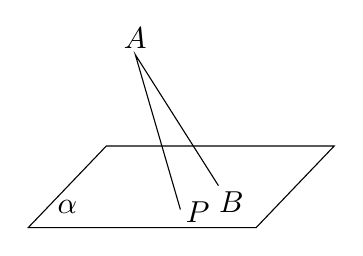
\begin{tikzpicture}[x=1pt, y=1pt,
    every node/.style={inner sep=0pt, font=\fontsize{10.5pt}{12.6pt}\selectfont}]
  \draw[line width=0.398pt] (54.9929,6.5198)   -- (38.6929,62.5048)   -- (68.7409,15.1658);
  \draw[line width=0.398pt] (0.0000,0.0000)   -- (82.3470,0.0000)   -- (110.5530,29.4810)   -- (28.2050,29.4810)   -- cycle;

  \node[anchor=center] at (38.700,68.512) {$A$};  % 源中心 (578.70,536.99)
  \node[anchor=center] at (61.250,5.562) {$P$};  % 源中心 (601.25,474.04)
  \node[anchor=center] at (73.400,9.262) {$B$};  % 源中心 (613.40,477.74)
  \node[anchor=center] at (14.150,7.362) {$\alpha$};  % 源中心 (554.15,475.84)

\end{tikzpicture}
%
% 【自验结果】
%   探针：latexmk -pdfxe（待跑）。
